\documentclass[]{article}
\synctex = 1

\usepackage{algorithm}
\usepackage{algpseudocode}
\usepackage{amsmath}
\usepackage{amssymb}
\usepackage{amsthm}
\usepackage{caption}
\usepackage{comment}
\usepackage{dsfont} 
\usepackage{graphicx}
\usepackage{hyperref}

\usepackage{listings}
\usepackage{amssymb}
\usepackage{multirow}
\usepackage{ mathrsfs }
\usepackage{subcaption}
\usepackage[utf8]{inputenc}
\usepackage{url}

\newcommand*{\CNN}{\ensuremath{\mathsf{CNN}}}
\newcommand*{\K}{\ensuremath{\mathsf{Kaught22}}}
\newcommand*{\keras}{\ensuremath{\mathsf{Keras}}}
\newcommand*{\numpy}{\ensuremath{\mathsf{NumPy}}}
\newcommand*{\scipy}{\ensuremath{\mathsf{SciPy}}}
\newcommand*{\scikit}{\ensuremath{\mathsf{sckit-learn}}}
\newcommand*{\Theano}{\ensuremath{\mathsf{Theano}}}
\newcommand*{\Model}[1]{\ensuremath{\mathsf{Model}}:#1}
%opening
\title{COMP540: Final Project Report}
\author{Harsh Upadhyay (hu3), Suguman Bansal (sb55)}
\date{}
\begin{document}

\maketitle

\begin{abstract}

\end{abstract}

\section{Introduction}
TODO

\section{Classifier}
\label{Sec:Classifier}

\subsection{Classifier architecture}
In this section we describe the architecture of $\K$, our Convolutional Neural Network for image classification. 

\paragraph{Component Layers}
We use four different kinds of layers to build $\K$: Convolutional layers (CONV), Activation layers (ReLu), Pool layers (Pool), and Fully-Connected layers (FC). We describe each one of these in detail below:
\begin{itemize}
\item CONV layer: All our convolutional layers learn filters on two-dimensional kernels. In all our CONV layers, we use a kernel of size $3\times 3$. We increase the number of filters to learn as we move deeper into the hidden layers (move towards the output). The first convolutional layer, the INPUT layer, takes in an additional parameter that indicates the size of the input images. In our case, the input size if $3 \times 32 \times 32$. 

\item ReLu layer:  The ReLu layer applies an element-wise activation function on its input. In our case, the activation function transforms every value $x$ to $max(x,0)$. This results in a non-affine transformation of the input to the layer. 

\item  Pool layer: We use a Pool layer to downsample the input size.  All our Pool layers down-sample each non-overlapping stride of dimension $2 \times 2$ to a single value that corresponds to the maximum of all values in the stride. This is called MaxPooling. 

\item FC layer: The fully connected layer is the usual neural network layer. It takes in as parameter the value of the number of outputs. We use FC layers only at the end of the architecture. 
\end{itemize}
The CONV and FC layers are trained with Nesterov's gradient descent~\cite{nesterov2012efficiency}, a variation of standard gradient descent with fast convergence,  with fixed hyper-parameters (Section~\ref{Sec:Implementation}). 

\paragraph{Component Blocks}
The architecture of $\K$ can be broken into two kinds of building blocks, where each building block is an arrangement of layers:
CONV blocks and FC blocks. 

\begin{itemize}
\item CONV Block: Each CONV block consists of 2 CONV layers, 2 ReLu activation layers, and one Pool layer. The architecture of a CONV Block is 
\[
[\text{CONV} -\text{ReLu} - \text{CONV} - \text{ReLu} - \text{Pool}]
\]
Each block is regularized with Dropout. Dropout regularization occurs only after transformations from the earlier 5 layers. The parameters on a CONV Block are the number of filters for the first and second CONV layers, and the dropout ratio. Therefore, CONV$(n_1, n_2, r)$ denotes a CONV Block with $n_1$ filters for the first CONV layer, $n_2$ filters for the second CONV layer, and dropout ratio $r$.

\item FC Block: Each FC block consists of a single FC layer. The parameters to an FC Block are  the number of output classes, and the activation function for the layer. An FC Block may or may not be regularized with dropout. FC$(o_1, act, r)$ denotes an FC block with $o_1$ number of output classes, $act$ activation function and a dropout ratio of $r$. In cases when $r$ is missing, we assign $r = 0$, indicating the absence of dropout regularization. 
\end{itemize}

\paragraph{$\K$ architecture}
$\K$ aligns 3 CONV blocks, with varying parameters, and follows them up with 2 FC blocks. The architecture for $\K$ is

\[
\text{CONV}(32, 64, 0.2)-\text{CONV}(64, 64, 0.2) - \text{CONV}(128, 64, 0.2) -\]
\[ - \text{FC}(256, \text{ReLu}, 0.5) - \text{FC}(10, \text{SoftMax})
\]
 

\begin{figure}[t]
\centering
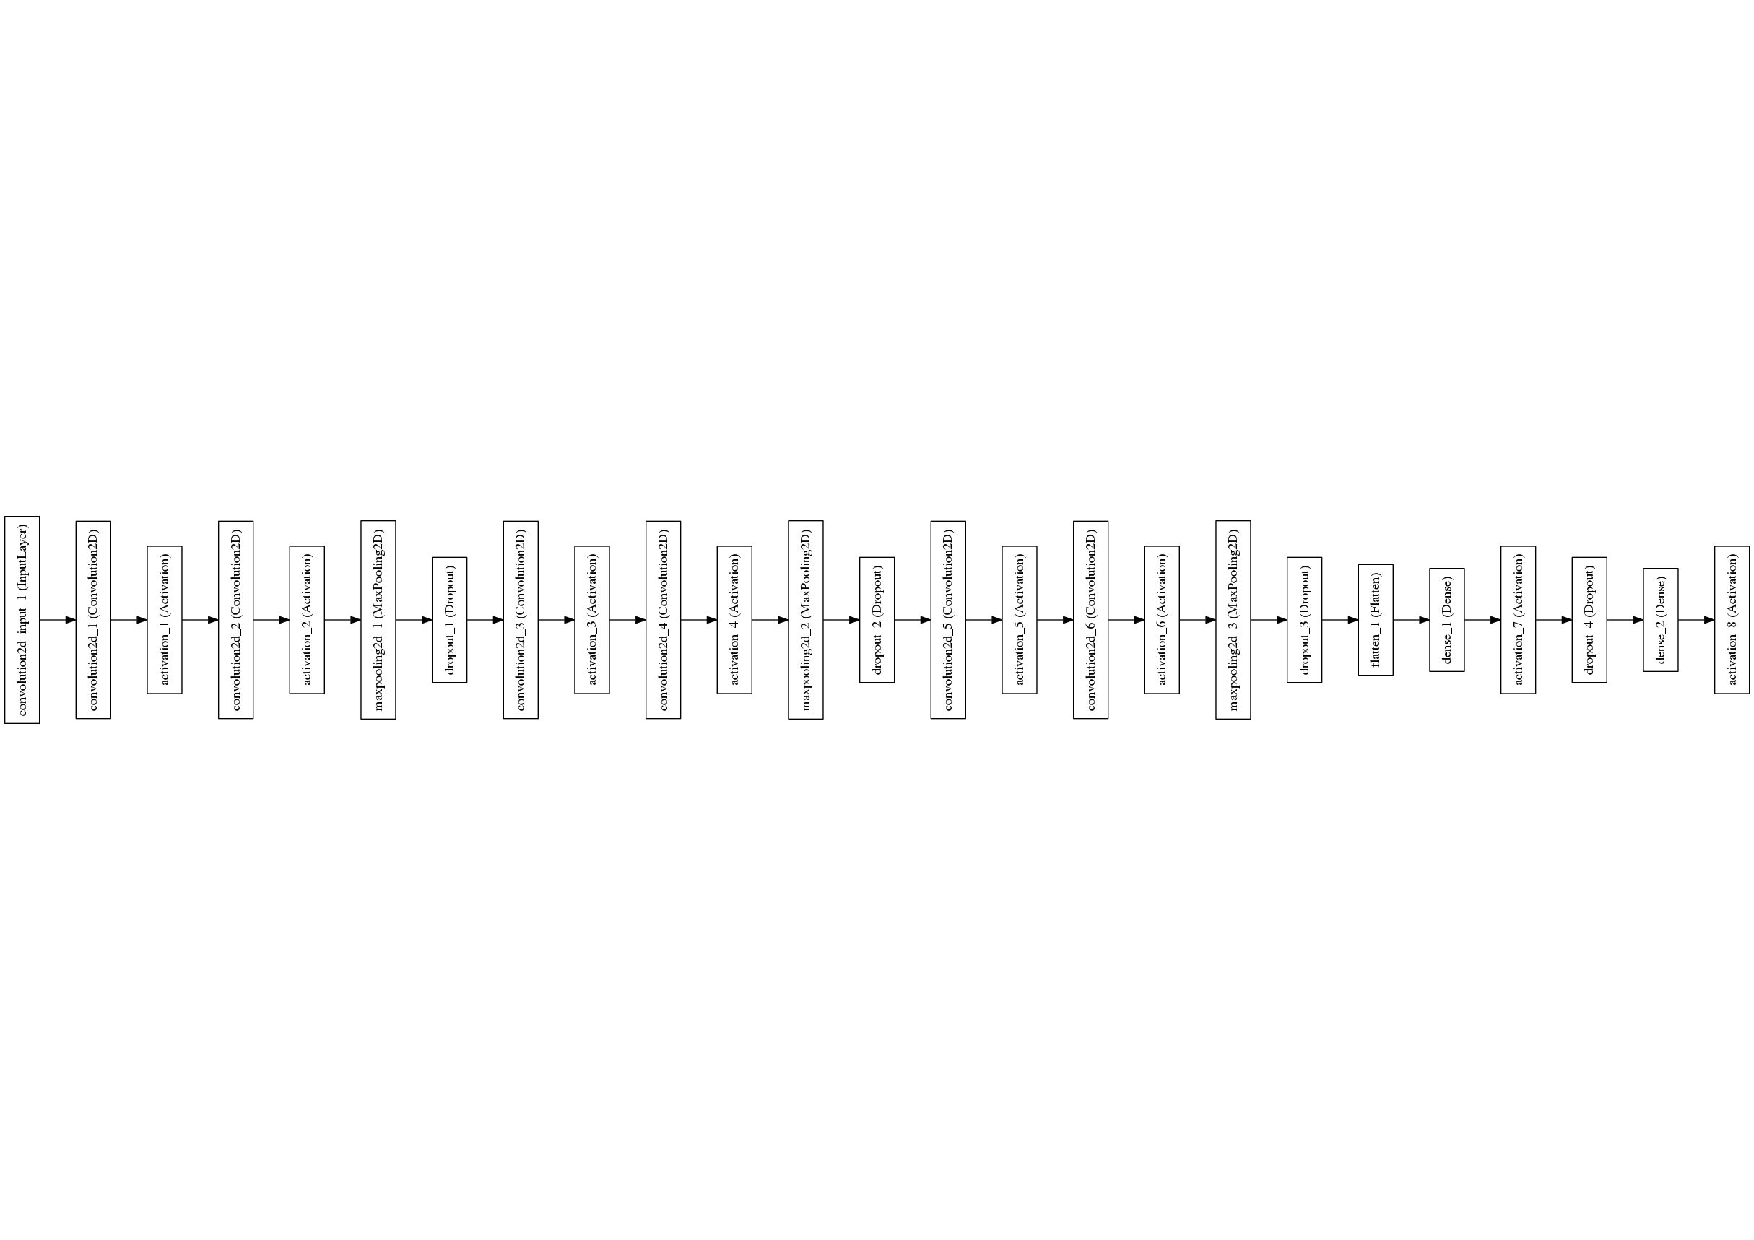
\includegraphics[width=\textwidth, trim={0, 8cm, 0, 8cm}]{model1.pdf}
\label{Fig:Model}
\caption{$\K$ Architecture}
\end{figure}
The detailed model architecture design is provided in Figure~\ref{Fig:Model}. The input to this network are images of dimension $3\times 32\times 32$. Due to MaxPool downsampling in each block, the output dimension after the third CONV block is $3 \times 4 \times 4$. This output is flattened (Flatten layer in Figure~\ref{Fig:Model}) before inserting it into the first FC block. The last FC block classifies the images into one of the 10 classes using a SoftMax classifier.  FC layers are shown as Dense layers in Figure~\ref{Fig:Model}. 




\subsection{Implementation details}
\label{Sec:Implementation}
We implemented our $\CNN$ classifier $\K$ on $\mathsf{Python}$ distribution circulated by $\mathsf{Anaconda}$. using the $\keras$~\cite{chollet2015keras} python library for neural network operations. We chose $\keras$  as our neural network library since it  builds on top of the $\Theano$~\cite{bergstra+al:2010-scipy, Bastien-Theano-2012} backend, which not only evaluates mathematical expressions involving multi-dimensional array efficiently,  but also leverages GPU capabilities very efficiently. 

\paragraph{Data Preprocessing}
To avoid repeated image reads, we save the data sets as a pickle.
We use $\mathsf{skimage.imread()}$ to read the data sets. We reshaped the data into $m\times 3\times 32 \times 32$, where $m$ is the size of the data sets, to maintain compatibility with the $\keras$ default.

We did not perform any mean shifting or standard deviation correction while reading the image, since $\keras$ allows the option to perform such operations on the fly while training and testing. This makes our code more dynamic for experimentation. 

We perform data preprocessing on the fly, as supported by $\keras$. First, we scale all the inputs between 0 and 1 by dividing each value in the training and testing dataset by 255.  In addition, we linearly shift the training data set by the value of the mean of the entire data set. Accordingly, we shift the  testing dataset with the same value as well. 

In addition to the above manual linear transformations,  we employ $\keras$'s in-built data augmentation option before feeding the train and test datasets to our model. In particular we shift the image by 10\% both in the vertical and horizontal direction, and we randomly flip the images along their vertical or horizontal axes. 


\paragraph{Hyper-parameter selection}
While training, we maintain a static ratio of 0.98 to split the training dataset into training and validation sets.  Currently, we are not shuffling the training dataset before spliting it into training and validation sets. 

We train our model for as many as 300 epochs. We utilize the entire data set of 50000 images per epoch, with a batch size of 32 images. 

We train weights in the model using standard gradient descent. To achieve faster convergence, we applied Nesterov's gradient descent~\cite{nesterov2012efficiency}. We set the learning rate to 0.01, decay rate to $10^{-6}$, and fix the momentum to 0.9. 


\paragraph{Recordings}
We maintained various parameters to perform sanity checks during the training processes. For each epoch run, we recorded the value of the loss function and accuracy for the training data and the validation data.  These values allowed us to estimate how well/poor the model would perform before completion of all epoch runs. This way, we could terminate the learning process before training would complete. 

We also stored the learnt weights periodically, so that we could analyze the weights in cases when we terminated before completion. 

\paragraph{Code Source}
You may find our source code at the link posted below:

 \url{https://github.com/HarshUpadhyay/COMP540_Project}
\section{Experimental evaluation}

\subsection{Experimental setup}
To harness GPU capabilities for linear algebra and vector operations, we ran our experiments on an Amazon Elastic Compute instance (EC2). The machine was of type  g2.2xlarge, backed by a single Nvidia GRID K520 GPU and an intel Xeon E5-2670 processor with 8x hardware hyperthreads and 15GiB RAM. The instance was running an Ubuntu server 14.04 LTS, with HVM virutalization support.

To achieve optimal performance from the machine, we compiled the $\mathsf{OpenBLAS}$ library to optimize $\numpy$ linear algebra performance. We also installed the latest $\mathsf{CUDA}$ drivers (Version 7.5) along with the $\mathsf{CuDNN}$ library, the bleeding edge version of $\mathsf{Theano}$,  and linked $\mathsf{Theano}$ with these libraries.

\begin{figure}[t]
\centering
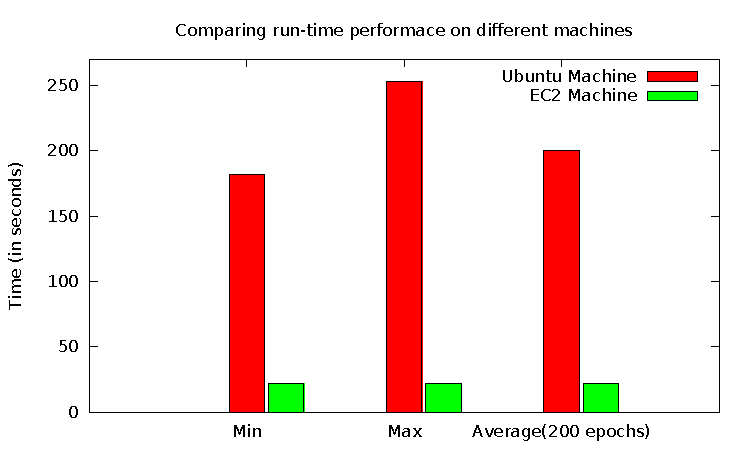
\includegraphics[scale=0.8]{Submissionlogs/RunTime.pdf}
\label{Fig:Runtime}
\caption{Comparing run-time on different machines}
\end{figure}

With the aforementioned set up, we observed a  drastic improvement of $\sim$10x in the runtime for training the model. In Figure~\ref{Fig:Runtime}, we compare the runtime performance while training the same model $\Model{1}$ (See Section~\ref{Sec:KaggleSub}) on two different machines. The EC2 machine in the figure corresponds to the server mentioned above. The Ubuntu machine refers to a standard Intel core i7, 2.8 GiHz machine on 8GiB RAM running on Ubuntu 14.04 LTS without GPU support. 






\subsection{Results}
\label{Sec:Results}
\subsubsection{Kaggle Submissions}
\label{Sec:KaggleSub}
So far, we have made 4 Kaggle submissions. In this section, we will discuss their architecture, performance on training and validation sets, and the Kaggle accuracy achieved on them. 

\paragraph{Architecture and Implementaion}
The main difference between the training process for first three models and $\K$, our fourth submission, is that in the first three we did not shift the train and test datasets with the mean of the training data set, whereas in $\K$ we do. Other differences between the model of $\K$ and earlier submissions are mentioned below:
\begin{itemize}
\item $\Model{1}$ - $\Model{1}$ shares the same architecture as $\K$, except that the dropout rate is set to 0.25 for all CONV Blocks. This is higher than the dropout rate in $\K$. $\Model{1}$ was trained on 200 epochs.
 
\item $\Model{2}$ - The architecture of $\Model{2}$ is richer than $\Model{1}$. We add another CONV Block, CONV$(128, 64, 0.25)$ to after the third CONV Block in $\Model{1}$. We compensate with the increase in number of parameters due to the additional block by reducing the number of outputs in the first FC Block to 128. The architecture for $\Model{2}$ is given below:
\[
\text{CONV}(32, 64, 0.25)-\text{CONV}(64, 64, 0.25) - \text{CONV}(128, 64, 0.25) -\]
\[ - \text{CONV}(128, 64, 0.25) - \text{FC}(128, \text{ReLu}, 0.5) - \text{FC}(10, \text{SoftMax})
\]
$\Model{2}$ was also trained on 200 epochs. 

\item $\Model{3}$ - $\Model{3}$ also shares the same architecture as $\K$, except that the dropout rate is set to a lower value of 0.125 for all CONV Blocks. Like $\K$,  $\Model{3}$ was trained on 300 epochs. 
\item $\K$: As described in Section~\ref{Sec:Classifier}.
\end{itemize} 

\paragraph{Accuracy and Loss performance}

\begin{table}[t]
\centering
\begin{tabular}{|c|c|c|c|}
\hline
            & \textbf{Training Accuracy} & \textbf{Validation Accuracy} & \textbf{Kaggle Accuracy} \\ \hline
$\Model{1}$ & 77.77                      & 82.20                        & 80.26                    \\ \hline
$\Model{2}$ & 75.87                      & 80.80                        & 79.73                    \\ \hline
$\Model{3}$ & 75.86                      & 79.90                        & 78.22                    \\ \hline
$\K$        & 95.53                      & 85.70                        & 84.32                    \\ \hline
\end{tabular}
\caption{Accuracy of Kaggle submissions}
\label{Tbl:Accuracy}
\end{table}

A comprehensive summary of the accuracy of all our Kaggle submissions is given in Table~\ref{Tbl:Accuracy}. The trends from the table indicate that addition of more layers results in diminishing returns, since the accuracy of $\Model{2}$ is lower than that of $\Model{1}$. Decline in accuracy of $\Model{3}$ indicates that a high dropout rate results in extreme regularization. Given these trends, we decided on a intermediate dropout rate for $\K$, and the optimal number of CONV Blocks of 3. Additionally, we observe that shifting data sets by the mean of the training data set drastically boosts the accuracy. 

More detailed trends of the accuracy while training are shown in Figure~\ref{Fig:AccKaggle}. From Figure~\ref{Fig:AccKaggle}, it is clear that in all cases, the accuracy trends on validation and training data sets were similar. In $\K$, we see that the model has become extremely optimized for the training data. As expected, in such a case we do not see an improvement in the accuracy of the validation set. 

\begin{figure}
\centering
\begin{minipage}{0.48\textwidth}
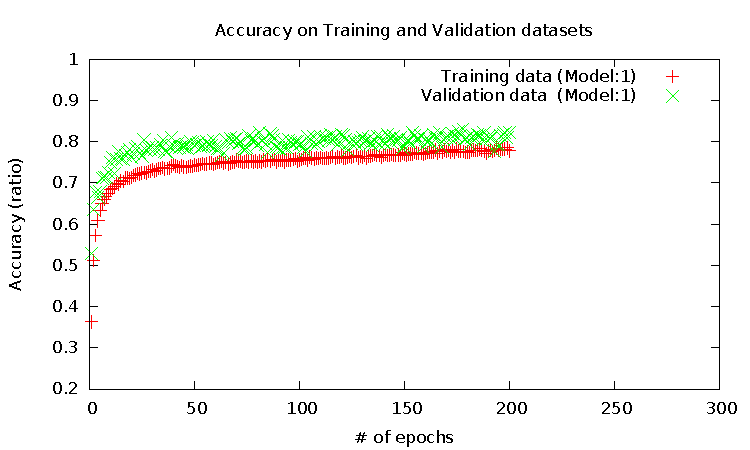
\includegraphics[scale=0.55, page=1]{Submissionlogs/LogAcc.pdf}
\end{minipage}
\hfill
\begin{minipage}{0.48\textwidth}
\includegraphics[scale=0.55, page=2]{Submissionlogs/LogAcc.pdf}
\end{minipage}
\hfill
\begin{minipage}{0.48\textwidth}
\includegraphics[scale=0.55, page=3]{Submissionlogs/LogAcc.pdf}
\end{minipage}
\hfill
\begin{minipage}{0.48\textwidth}
\includegraphics[scale=0.55, page=4]{Submissionlogs/LogAcc.pdf}
\end{minipage}
\caption{Trends of Accuracy on training and validation data sets on all models}
\label{Fig:AccKaggle}
\end{figure}

More detailed trends of the loss function while training are shown in Figure~\ref{Fig:LossKaggle}. The inferences from the trends of the loss function on the validation and training set of the models are identical to that from the accuracy. 

\begin{figure}
\centering
\begin{minipage}{0.48\textwidth}
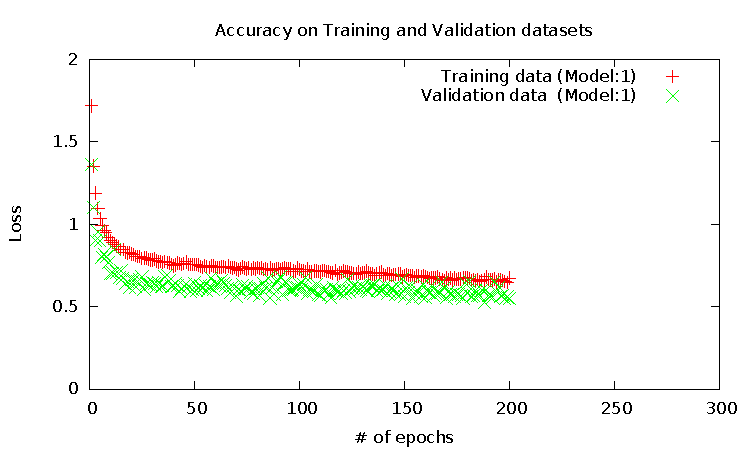
\includegraphics[scale=0.55, page=1]{Submissionlogs/LogLoss.pdf}
\end{minipage}
\hfill
\begin{minipage}{0.48\textwidth}
\includegraphics[scale=0.55, page=2]{Submissionlogs/LogLoss.pdf}
\end{minipage}
\hfill
\begin{minipage}{0.48\textwidth}
\includegraphics[scale=0.55, page=3]{Submissionlogs/LogLoss.pdf}
\end{minipage}
\hfill
\begin{minipage}{0.48\textwidth}
\includegraphics[scale=0.55, page=4]{Submissionlogs/LogLoss.pdf}
\end{minipage}
\caption{Trends of Loss function on training and validation data sets on all models}
\label{Fig:LossKaggle}
\end{figure}

In summary, of all our Kaggle submissions, our best was obtained on $\K$, which performs mean shifting, its architecture comprises of 3 CONV Blocks and two FC Blocks, and an intermediate dropout rate for regularization. 

\subsubsection{Other notable results}
We experimented a lot with hyper-parameters. Here we summarize the architecture, results, and inferences from some un-successful experiments which lead to important insights. 

\paragraph{Increasing number of CONV Blocks}
We noticed that increasing the number of CONV Block and increasing the number of outputs for the first FC Block did not result in any accuracy improvement. Figure~\ref{Fig:AccMoreLayers} depicts the trends of accuracy when the model architecure is similar to that of $\Model{2}$ with different parameters for the first FC block. The parameters on the first FC block in models shown in Figure~\ref{Fig:AccMoreLayers} are FC(256, 0.5) and FC(512. 0.5). 

We suspect that the observed trend occurs since the number of parameters is vary large as compared to the amount of data provided. This is a case of under-fitting. 
\begin{figure}
\centering
\begin{minipage}{0.48\textwidth}
\includegraphics[scale=0.55, page=6]{Submissionlogs/LogAcc.pdf}
\end{minipage}
\hfill
\begin{minipage}{0.48\textwidth}
\includegraphics[scale=0.55, page=7]{Submissionlogs/LogAcc.pdf}
\end{minipage}
\caption{Trends of accuracy with more layers}
\label{Fig:AccMoreLayers}
\end{figure}


\paragraph{Mean shift and standard deviation correction of individual images}
We experimented with data augmentation options provided by $\keras$. $\keras$ provides an option to center every image at 0 by shifting it by its own mean value, and correcting its standard deviation so that it becomes 1. In this case, each image is transformed with its own parameters. In our experiments with zero-centering and standard deviation correction, we observed extreme over-fiting. While the accuracy on the training data set went to as high as 70\%, validation accuracy was often stranded at around 15\%.  

%attempts folders are the ones we tried yesterday with data augmentations and droupout=0.125 for the last one I think 
%one was with stat correction off
%one was with stat correction on


\subsection{Obsevations}
\begin{enumerate}
\item We benefited from running our experiments on EC2 as it drastically reduced the computation time. Not only did this enable us to perform more experiments, but we could also increase the number of epochs by 50\%.
\item We observe that shifting the images with the mean of the training data enhances the accuracy significantly.
\item Addition of too many layers results in under-fiting, as expected. 
\item Aggressive regularization with too high dropout rate, and meek regularization with low dropout rate reduces the accuracy. An intermediate dropout rate seems optimal from our experiments. 
\item Image-wise zero-centering, and standard deviation correction results in over-fitting. 
\item Flipping images randomly along an axis makes the learning process more sturdy. 
\end{enumerate}
	
\section{Previous attempts}
In our earlier attempts, we worked with scikit-neuralnetworks. However, since the library did not provide seamless GPU support, we were not able to perform fast learning. We had to stop learning after a few epochs only, since each epoch took very long to complete computation. Hence, we decided to move to $\keras$ library for CNN support. 

We used our personal computers with $\keras$ initially. However, as we moved on to CNNs, even on these computers each epoch would take extremely long. Hence, we eventually shifted our experimental set up EC2, where we could exploit the benefit of GPU (See Figure~\ref{Fig:Runtime}).


\section{Future Work}
An interesting future direction would be to set up an ensemble of these CNNs to classify images.
\section*{Acknowledgements}
We acknowledge insightful discussion with various classmates namely Jack Fesser and Lucas Tabajara.

\section{Comments}
correction:
"input size is 3x32x32" ? in the classifier section
Shouldn't it be 
"Our network accepts a vector of dimensions mx3x32x32
should we use "our network" or "our implementation" instead of "in our case" each time
Architecture - we have 2 CONV blocks
3 par vo underfit wala graph aaya tha
Correct one:
 
CONV(32;  32;  0: 2) 􀀀  CONV(64;  64;  0: 2) 􀀀􀀀
􀀀 FC(512);  ReLu;  0: 5) 􀀀  FC(10;  SoftMax)
check the latest utils.py that I sent along with our best entry
and I did not use Anaconda lol
Typo in data preprocessing section:
"  We reshaped the
data into m   3   32   32, where m  is the size of the data sets,"
data sets is wrong we have one data set
Also, I checked that I had my learning rate to 0.001 which is 1/10 of the default
latest accuracy is 0.84630 when I ran for fewer epochs(265 instead of 300)
also - sorry for miscommunication too many parameters means overfitting
my bad
basically har baar overfitting hi hui hai - never underfit
baki sab toh theek hi hai
maybe it can pass off as a draft
\bibliographystyle{plain}
\bibliography{refs}

\end{document}
